\chapter{Bewertung und Diskussion} %Kapitelüberschriften
\label{chap5}
In den vorigen Kapiteln wurden technische Daten zu Ladesystemen, Speichersystemen und deren Kombinationen erhoben und berechnet. In diesem Kapitel wird nun eine gewichtete Bewertung dieser Kriterien erstellt, um Vor- und Nachteile der verschiedenen Gesamtsysteme betrachten zu können.

Die Systeme werden aus rein technischer Sicht betrachtet, wirtschaftliche Aspekte wurden in dieser Arbeit noch nicht einbezogen. Von daher sollte diese Bewertung letztlich im Zusammenhang mit einer Analyse aus wirtschaftlicher Sicht betrachtet werden. Die hier durchgeführte technische Analyse und Bewertung liefert die Grundlage für eine solche wirtschaftliche Analyse.

\section{Gewichtete Bewertung}
Im vorigen Kapitel wurden die Werte 6 verschiedener Parameter für alle Kombinationen von fünf Batterien, insgesamt fünf Ladesystemen und zwei Buslinien berechnet. So sind  Datenpunkte entstanden. Diese Menge muss nun mit einem geeigneten Verfahren auf wenige Kennwerte reduziert werden, mit denen die Eignung einer bestimmten Kombination von Ladestrategie, Ladesystem und Speichertechnologie für eine bestimmte Strecke bestimmt werden kann.

Dazu wurde die Methode der gewichteten technischen Bewertung nach VDI~2225 Blatt~3~\cite{vdi:2225} gewählt. Diese besteht aus vier Phasen:
\begin{enumerate}
	\item Festlegung der Parameter und Mindestanforderungen
	\item Zuordnung von Punktzahlen zu Leistungsmerkmalen
	\item Gewichtung der Punktzahlen
	\item Berechnung der gewichteten Mittelwerte
\end{enumerate}

\subsection{Festlegung der Parameter und Mindestanforderungen}
Die Festlegung der Parameter ist bereits in den Abschnitten \ref{parameterDirekt} und \ref{simErgebnisse} erfolgt. Die Erfüllung der Mindestanforderungen hinsichtlich Stromstärke und Energie wurden durch die Optimierung der Batteriegröße sichergestellt.

Um bei einer maximalen Fahrzeugmasse von 18 Tonnen und einem Leergewicht von 13 Tonnen mindestens 50 Passagiere mit einem Gesicht von jeweils 68 kg transportieren zu können, darf das Gewicht von Batterie und Ladesystem 1,6 Tonnen nicht überschreiten. Wie in den Tabellen \ref{204_a} und \ref{192_a} zu sehen, wird diese Anforderung wird von der Bleibatterie für keine Kombination erfüllt, von daher wird die Bleibatterie nicht weiter betrachtet. Der Lithium-Titanat-Akku und der Lithium-Eisenphosphat-Hochleistungsakku sind für bestimmte Kombinationen nicht geeignet. Diese Kombinationen werden mit "`unbefriedigend"' bewertet.

\subsection{Zuordnung von Punktzahlen}
Zur Bewertung werden die Kriterien aus Abschnitt \ref{parameterDirekt} und \ref{simErgebnisse} verwendet. Die Massen von Ladesystem und Batterie sowie das Batterievolumen und das freie Volumen des Ladesystems werden zu einem Gesamtvolumen und einer Gesamtmasse zusammengefasst.

Die Zuordnung der Punkte erfolgt anhand einer subjektiven Bewertung der Güte eines bestimmten Wertebereichs. Die Bewertungen der Punkte sind in Tabelle \ref{tabPunkte} dargestellt. Es wird darauf geachtet, das der Durchschnittswert der Punktzahlen der technisch akzeptablen Lösungen bei ca. 2,5 liegt.

\begin{table} \centering
	\begin{tabular}{rl}
		\toprule
		Punktzahl & Bewertung           \\ \midrule
		        0 & unbefriedigend      \\
		        1 & gerade noch tragbar \\
		        2 & ausreichen          \\
		        3 & gut                 \\
		        4 & sehr gut            \\ \bottomrule
	\end{tabular}
	\caption[Bewertung der Punktzahlen]{Bewertung der Punktzahlen nach VDI~2225 Blatt~3~\cite{vdi:2225}[S. 5]}
	\label{tabPunkte}
\end{table}

Auf Basis des in Tabelle \ref{tabPunkte} dargestellten Schemas wurden den in der Simulation berechneten Werten Punktzahlen zugeordnet. Sie sind in Tabelle \ref{tab_punktzahlen} aufgeführt.

\begin{table}
	\centering
	\begin{tabulary}{\linewidth}{LLrrrr}
		\toprule
		Kriterium                                                & Einheit              &         1P &      2P &        3P &           4P \\ \midrule
		\textbf{Zuverlässigkeit Fahrzeug}                        &                      &            &         &           &  \\
		Ladezyklen pro tausend Kilometer                         & $\frac{1}{10^{3}km}$ &   $\ge 30$ &   $<30$ &     $<10$ &         $<5$ \\
		Masse Ladesystem + Batterie                              & kg                   & $\ge 1250$ & $<1250$ &    $<750$ &       $<250$ \\
		Positionierungsgenauigkeit (Fläche)                      & $m^2$                &       $<3$ &    $<6$ &      $<9$ &      $\ge 9$ \\
		Freiheitsgrade Ladesystem Fahrzeug                       & 1                    &       $>2$ &       2 &         1 &            0 \\
		Positionierungsgenauigkeit (Winkel)                      & $^\circ$             &       $<5$ &     --- &       --- &        $360$ \\
		Zugänglichkeit Schnittstelle Fahrzeug                    & ---                  &        --- &   Seite &     Boden &         Dach \\ \midrule
		\textbf{Störanfälligkeit der Ladestation}                &                      &            &         &           &  \\
		Zeiteffizienz                                            & 1                    &     $<0,6$ & $<0,75$ &    $<0,9$ &    $\ge 0,9$ \\
		Exponierte Leiter                                        & ---                  &      immer &     --- & nur Laden &          nie \\
		Zugänglichkeit Ladestation                               & ---                  &  ebenerdig &  erhöht & unterflur & unzugänglich \\ \midrule
		\textbf{Verfügbarkeit von elektrischen Niederflurbussen} &                      &            &         &           &  \\
		Volumen Ladesystem (feste Position)                      & l                    & $\ge 1000$ & $<1000$ &    $<500$ &       $<250$ \\
		Volumen Ladesystem freie Position + Volumen Batterie     & l                    &  $\ge 400$ &  $<400$ &    $<200$ &       $<100$ \\ \midrule
		\textbf{Vermeidung von CO\textsubscript{2}-Emissionen}   &                      &            &         &           &  \\
		Energieverbrauch                                         & $\frac{kWh}{km}$     &  $\ge 1,5$ &  $<1,5$ &    $<1,2$ &       $<0,9$ \\ \midrule
		\textbf{Einsatz unter extrem Umweltbedingungen}          &                      &            &         &           &  \\
		Kühlluftmasse                                            & $\frac{g}{s}$        & $\ge 5000$ & $<5000$ &   $<3000$ &      $<1000$ \\ \bottomrule
	\end{tabulary}
	\caption[Zuordnung von Punktzahlen zu den Ergebnissen]{Zuordnung von Punktzahlen zu den Ergebnissen}
	\label{tab_punktzahlen}
\end{table} 

\subsection{Gewichtung der Punktzahlen}
Tabelle \ref{tab_punktzahlen} erlaubt die eindeutige Zuordnung von Punktzahlen für die berechneten Parameter. Da die verschiedenen Parameter aber offensichtlich von unterschiedlicher Wichtigkeit sind, wird in dieser Arbeit anschließend noch eine Gewichtung vorgenommen.

Die Auswahl und Gewichtung der Bewertungskriterien basiert auf der Masterarbeit von Thomas Pannwitz, in der eine Umfrage unter 17 Busbetreibern über ihre Entscheidungskriterien für die Busbeschaffung durchgeführt wurde. Die fünf wichtigsten Anforderungen der Busbetreiber waren~\cite{pannwitz2014}[S. 25]:
\begin{enumerate}
	\item hohe technische Zuverlässigkeit des Fahrzeugs
	\item geringe Störanfälligkeit der Ladestation
	\item Verfügbarkeit von elektrischen Niederflurbussen
	\item Vermeidung von $CO_2$-Emissionen
	\item effizienter Einsatz unter extrem Umweltbedingungen
\end{enumerate}

Auf Basis dieser Kriterien wurden die in Tabelle \ref{tab_bewertungskriterien} dargestellte Gewichtungsschemata entwickelt. Die Gewichtung der Parameter wurde im ersten Schema entsprechend den genannten Anforderungen der Busbetreiber festgelegt. Da die relativen Unterschiede der Gewichtungen in der Umfrage nicht signifikant waren, wurde ein alternatives Gewichtungsschema mit gleichen Gewichtungen für die unterschiedlichen Kategorien erstellt. Parameter, die sich nicht eindeutig unter einer der genannten Anforderungen einsortieren liessen wurden bestmöglich einsortiert
\begin{table}
	\centering
	\begin{tabulary}{\linewidth}{LRLL}
		\toprule
		Kriterium                                                &                   & Gewichtung (\%) & Alternative Gewichtung (\%) \\ \midrule
		\textbf{Zuverlässigkeit Fahrzeug}                        &                   &                 &  \\
		Ladezyklen pro tausend Kilometer                         &                   & 8               & 3,3                         \\
		Masse Ladesystem + Batterie                              &                   & 6               & 3,3                         \\
		Positionierungsgenauigkeit (Fläche)                      &                   & 6               & 3,3                         \\
		Freiheitsgrade Ladesystem Fahrzeug                       &                   & 4               & 3,3                         \\
		Positionierungsgenauigkeit (Winkel)                      &                   & 3               & 3,3                         \\
		Zugänglichkeit Schnittstelle Fahrzeug                    &                   & 3               & 3,3                         \\ \midrule
		                                                         &          $\Sigma$ & \textbf{30}     & \textbf{20}                 \\
		\textbf{Störanfälligkeit der Ladestation}                &                   &                 &  \\
		Zeiteffizienz                                            &                   & 15              & 6,7                         \\
		Exponierte Leiter                                        &                   & 5               & 6,7                         \\
		Zungänglichkeit Ladestation                              &                   & 5               & 6,7                         \\ \midrule
		                                                         &          $\Sigma$ & \textbf{25}     & \textbf{20}                 \\
		\textbf{Verfügbarkeit von elektrischen Niederflurbussen} &                   &                 &  \\
		Volumen Ladesystem (feste Position)                      &                   & 10              & 10                          \\
		Volumen Ladesystem (freie Position) + Volumen Batterie   &                   & 10              & 10                          \\ \midrule
		                                                         &          $\Sigma$ & \textbf{20}     & \textbf{20}                 \\
		\textbf{Vermeidung von CO\textsubscript{2}-Emissionen}   &                   &                 &  \\
		Energieverbrauch                                         &                   & 15              & 20                          \\ \midrule
		                                                         &          $\Sigma$ & \textbf{15}     & \textbf{20}                 \\
		\textbf{Einsatz unter extrem Umweltbedingungen}          &                   &                 &  \\
		Kühlluftmasse                                            &                   & 10              & 20                          \\ \midrule
		                                                         &          $\Sigma$ & \textbf{10}     & \textbf{20}                 \\ \midrule
		                                                         & $\Sigma_{gesamt}$ & 100             & 100 \\ \bottomrule
		                                                         &
	\end{tabulary}
	\caption{Gewichtung der Bewertungskriterien der Gesamtlösungen}
	\label{tab_bewertungskriterien}
\end{table} 

\subsection{Ergebnisse der gewichteten Bewertung}
In Abbildung \ref{abb_DiagrammAuswertung} sind die Ergebnisse der gewichteten Bewertungen grafisch dargestellt. Die Zahlenwerte der Bewertung mit der ersten Gewichtung sind in den Tabellen \ref{tab_ergebnisse204} und \ref{tab_ergebnisse192} zu sehen. Die Ergebnisse für die alternative Gewichtung sind in den Tabellen \ref{tab_ergebnisse204a} und \ref{tab_ergebnisse192a} aufgeführt. Neben dem gewichteten Mittelwert zu jeder Kombination von Ladesystem und Speichertechnologie sind in den Tabellen Durchschnittswerte für ein Ladesystem bzw. eine Speichertechnologie und Linie berechnet worden.

\paragraph{Digitaler Anhang} In Anhang \ref{an_Digital} ist die zur Berechnung verwendete Tabelle enthalten. Sie ist unter dem Namen \texttt{Auswertung.ods} zu finden und kann mit \textsc{LibreOffice} geöffnet werden.

\begin{figure}\centering
	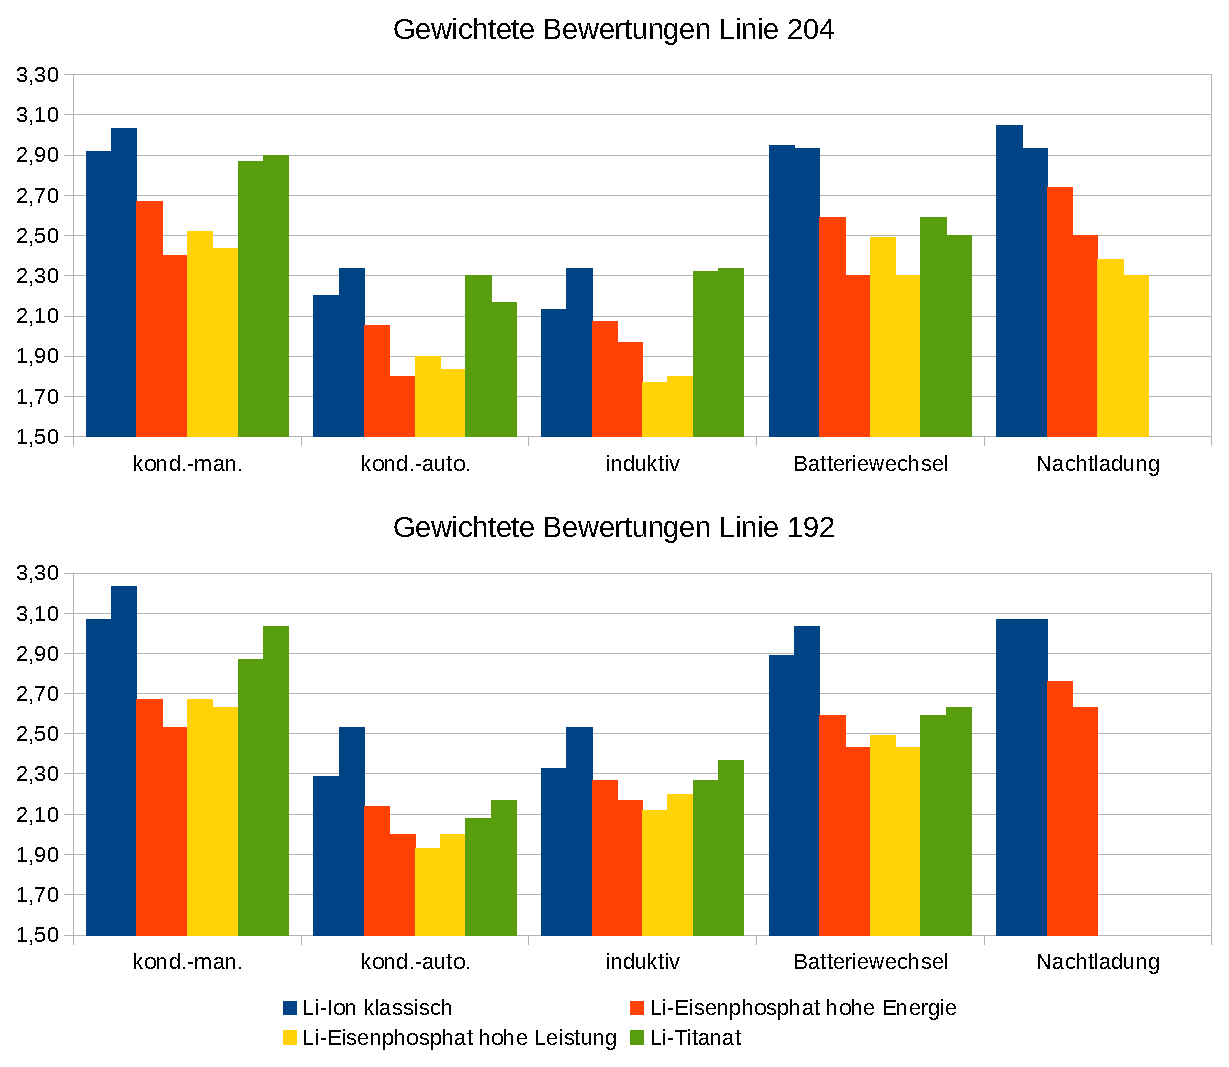
\includegraphics[width=\myFigureWideWidth]{DiagrammeAuswertung}
	\caption[Diagramm der gewichteten Bewertungen]{Diagramm der gewichteten Bewertungen. Der linke Balken einer Farbe stellt das Ergebnis für das erste Gewichtungsschema dar, der rechte Balken ist das Ergebnis für das alternative Gewichtungsschema.}
	\label{abb_DiagrammAuswertung}
\end{figure}

\begin{table} \centering
	\begin{tabulary}{\linewidth}{LRRRRRR}
		\toprule
		Bat./LS                          &         \multicolumn{4}{c}{Gelegenheitsladen}         & \multicolumn{1}{c}{Nachtladung} & Zeilen-$\varnothing$ \\
		\cmidrule{2-5}                   &    kond.-man. & kond.-auto. & indu. & Batteriewechsel &               konduktiv-manuell &  \\ \midrule
		"`klassischer"' Li-Ionen-Akku    & \textbf{2,92} &        2,20 &  2,13 &   \textbf{2,95} &                   \textbf{3,05} &                 2,65 \\
		Li-Eisenphosphat (hohe Energie)  &          2,67 &        2,05 &  2,07 &            2,59 &                   \textbf{2,74} &                 2,42 \\
		Li-Eisenphosphat (hohe Leistung) &          2,52 &        1,90 &  1,77 &            2,49 &                            2,38 &                 2,21 \\
		Lithium-Titanat                  & \textbf{2,87} &        2,30 &  2,32 &            2,59 &                             --- &                 2,52 \\
		Spalten-$\varnothing$            &          2,75 &        2,11 &  2,07 &            2,66 &                            2,72 &  \\ \bottomrule
	\end{tabulary}
	\caption[Ergebnisse der Simulation Linie 204 mit erster Gewichtung]{Ergebnisse der Simulation Linie 204 mit erster Gewichtung. Die Bewertungen liegen zwischen 1 (schlechteste Bewertung) und 4 (beste Bewertung). Die fünf besten Werte sind markiert. Ungeeignete Systeme wurden ausgelassen.}
	\label{tab_ergebnisse204}
	
	
	\begin{tabulary}{\linewidth}{LRRRRRR}
		                                 &               &               &       &                 &                                 &  \\ \toprule
		Bat./LS                          &          \multicolumn{4}{c}{Gelegenheitsladen}          & \multicolumn{1}{c}{Nachtladung} & Zeilen-$\varnothing$ \\
		\cmidrule{2-5}                   &    kond.-man. &   kond.-auto. & indu. & Batteriewechsel &               konduktiv-manuell &  \\ \midrule
		"`klassischer"' Li-Ionen-Akku    & \textbf{3,07} & 2,29          &  2,33 &   \textbf{2,89} &                  \textbf{ 3,07} &                 2,73 \\
		Li-Eisenphosphat (hohe Energie)  &          2,67 &          2,14 &  2,27 &            2,59 &                  \textbf{2,76} &                 2,49 \\
		Li-Eisenphosphat (hohe Leistung) &          2,67 &          1,93 &  2,12 &            2,49 &                             --- &                 2,30 \\
		Lithium-Titanat                  & \textbf{2,87} &          2,08 &  2,27 &            2,59 &                             --- &                 2,45 \\
		Spalten-$\varnothing$            &          2,82 &          2,11 &  2,25 &            2,64 &                            2,92 &  \\ \bottomrule
	\end{tabulary}
	\caption[Ergebnisse der Simulation Linie 192 mit erster Gewichtung]{Ergebnisse der Simulation Linie 192 mit erster Gewichtung. Die Bewertungen liegen zwischen 1 (schlechteste Bewertung) und 4 (beste Bewertung). Die fünf besten Werte sind markiert. Ungeeignete Systeme wurden ausgelassen.}
	\label{tab_ergebnisse192}
\end{table}

\begin{table} \centering
	\begin{tabulary}{\linewidth}{LRRRRRR}
		\toprule
		Bat./LS                          &         \multicolumn{4}{c}{Gelegenheitsladen}         & \multicolumn{1}{c}{Nachtladung} & Zeilen-$\varnothing$ \\
		\cmidrule{2-5}                   &    kond.-man. & kond.-auto. & indu. & Batteriewechsel &               konduktiv-manuell &  \\ \midrule
		"`klassischer"' Li-Ionen-Akku    & \textbf{3,03} & 2,33        &  2,33 &   \textbf{2,93} &                   \textbf{2,93} &                 2,71 \\
		Li-Eisenphosphat (hohe Energie)  &          2,40 &        1,80 &  1,97 &            2,30 &                   \textbf{2,50} &                 2,19 \\
		Li-Eisenphosphat (hohe Leistung) &          2,43 &        1,83 &  1,80 &            2,30 &                            2,30 &                 2,13 \\
		Lithium-Titanat                  & \textbf{2,90} &        2,17 &  2,33 &   \textbf{2,50} &                             --- &                 2,47 \\
		Spalten-$\varnothing$            &          2,69 &        2,03 &  2,11 &            2,51 &                            2,58 &  \\ \bottomrule
	\end{tabulary}
	\caption[Ergebnisse der Simulation Linie 204 mit alternativer Gewichtung]{Ergebnisse der Simulation Linie 204 mit alternativer Gewichtung. Die Bewertungen liegen zwischen 1 (schlechteste Bewertung) und 4 (beste Bewertung). Die fünf besten Werte sind markiert. Ungeeignete Systeme wurden ausgelassen.}
	\label{tab_ergebnisse204a}
	
	
	\begin{tabulary}{\linewidth}{LRRRRRR}
		&               &               &       &                 &                                 &  \\ \toprule
		Bat./LS                          &          \multicolumn{4}{c}{Gelegenheitsladen}          & \multicolumn{1}{c}{Nachtladung} & Zeilen-$\varnothing$ \\
		\cmidrule{2-5}                   &    kond.-man. &   kond.-auto. & indu. & Batteriewechsel &               konduktiv-manuell &  \\ \midrule
		"`klassischer"' Li-Ionen-Akku    & \textbf{3,23} & 2,53     &  2,53      &   \textbf{3,03} &                  \textbf{3,07}  &                 2,88 \\
		Li-Eisenphosphat (hohe Energie)  &          2,53 &          2,00 &  2,17 &            2,43 &                 \textbf{2,63} &                 2,35 \\
		Li-Eisenphosphat (hohe Leistung) &          2,63 &          2,00 &  2,20 &            2,43 &                             --- &                 2,32 \\
		Lithium-Titanat                  & \textbf{3,03} &          2,12 &  2,37 &   \textbf{2,63} &                             --- &                 2,55 \\
		Spalten-$\varnothing$            &          2,86 &          2,17 &  2,32 &            2,63 &                            2,85 &  \\ \bottomrule
	\end{tabulary}
	\caption[Ergebnisse der Simulation Linie 192 mit alternativer Gewichtung]{Ergebnisse der Simulation Linie 192 mit alternativer Gewichtung. Die Bewertungen liegen zwischen 1 (schlechteste Bewertung) und 4 (beste Bewertung). Die fünf besten Werte sind markiert. Ungeeignete Systeme wurden ausgelassen.}
	\label{tab_ergebnisse192a}
\end{table}

\section{Diskussion}
Die am besten bewerteten Kombinationen sind für beide Buslinien die Kombination von Lithium-Titanat-Batterie und konduktiv-manueller Aufladung sowie das Aufladen über Nacht mit Lithium-Schichtoxid-Batterien.

\paragraph{Konduktiv-Manuelles System bei Gelegenheitsladung} Das konduktiv-manuelle System ist das am besten bewertete Ladesystem für die Ladestrategie "`Gelegenheitsladung"'. Dies lässt sich durch den Fokus auf Zuverlässigkeit und Kompaktheit erklären. Dieses Ladesystem ist vergleichsweise einfach und leicht, es besitzt keine automatisch bewegten Teile und stellt keine hohen Anforderungen an die Position des Busses. Die Ladezeit beträgt zwischen 25 und 40 Minuten nach jeder Tour (Fahrzeiten 77 und 61 Minuten) und ist damit zwischen drei- und fünfmal länger als die des konduktiv-automatischen Systems. Für die gleiche Taktfrequenz werden daher mit dieser langsameren Technologie mehr Fahrzeuge und Fahrer benötigt, die erhöhte Kosten mit sich bringen. Für eine genauere Analyse ist neben den Kosten sämtlicher Komponenten also auch eine Betrachtung der gewünschten Taktfrequenz nötig.

\paragraph{Nachtladung} Die hohe Bewertung von Nachtladesystem (dreimal zweitbestes und einmal bestes System) widerspricht der anfänglichen Hypothese, das die benötigten schweren Batterien (0.7 - 1,5 t im Genesatz zu 0,2 - 0,7 t bei Gelegenheitsladung) nicht praxistauglich seien. Zwei der vier Batterien haben jedoch genug Kapazität, um auf beiden Linien einen Betriebstag mit 11 Umläufen zu überstehen. Auch der als möglicher Nachteil vermutete höhere Energieaufwand konnte in der Simulation nicht bestätigt werden. Es wird sogar der niedrigste Energieverbrauch auf beiden Buslinien erreicht. Dies lässt sich durch die bessere Rekuperationsleistung der Batterien erklären. Die spezifische Rekuperationsleistung hat sich in der Simulation das begrenzende Element erwiesen, und eine größere Batterie kann entsprechend mehr rekuperieren. Im Betrieb werden bei der Ladestrategie "`Nachtladung"' sogar weniger Fahrzeuge benötigt als bei jeder anderen Ladestrategie, da während des Betriebs tagsüber gar keine Ladezeit anfällt. Im Gegenzug sind die Fahrzeuge durch die großen Batterien in der Anschaffung erheblich teurer und durch das etwas höhere Gewicht verschleißen Fahrzeug und Straße eventuell schneller. Auch hier ist eine Betrachtung der geforderten Taktfrequenz nötig, auch die Verschleißkosten der Straßen für verschiedene Fahrzeuggewichte sollten betrachtet werden.

\paragraph{Batteriewechselsysteme} Das insgesamt am drittbesten bewertete Ladesystem ist das Wechseln der Batterien durch Roboter in einem speziellen Gebäude. Es zeichnet sich durch eine "`konstante"' Ladezeit aus, da die Batterie im Bus nach dem sieben Minuten langen Wechselvorgang unabhängig von ihrer Größe "`vollständig geladen"' ist. Daneben muss keine Ladeelektrik im Fahrzeug mitgeführt werden und die Batterien können außerhalb des Busses sehr effizient geladen werden. Allerdings ist die Ladestation sehr viel aufwändiger, da die Batterien  von Robotern entnommen und in Ladebuchten transportiert werden müssen. Von daher macht dieses System für den Einsatz von nur wenigen Elektrobussen keinen Sinn. Erst beim Einsatz einer großen Flotte wird die Investition in so ein aufwändigeres Ladesystem sinnvoll.

\paragraph{Kein Vorteil für Ladeleistungen über 200 kW} Das konduktiv-automatische Ladesystem mit 375 kW hat in fast jeder Kombination schlechter abgeschnitten als das induktive System mit 200 kW. Aufgrund der begrenzten Ladeleistung der Batterien hat die höhere Ladeleistung keinen Vorteil, selbst der Lithium-Titanat-Akku erreicht eine maximale Ladeleistung von ca. 170 kW. Aufgrund der größeren und exponierteren Komponenten und der größeren Anzahl an Komponenten des konduktiv-automatischen Systems wird eine höhere Fehleranfälligkeit erwartet. Der ca. 5\% niedrigere Energieverbrauch reichte in der Bewertung nicht aus, um die Nachteile auszugleichen. Durch den Einsatz einer größeren Batterie könnte auch mit aktueller Technologie eine Ladezeit von 5 Minuten pro Umlauf (statt 8 Minuten mit minimaler Batteriegröße) erreicht werden, dies würde jedoch eine fast doppelt so große und teure Batterie erfordern.

\paragraph{18650-Zelle} Die hohe Bewertung der Lithium-Schichtoxid-Batterien zeigt, das Batterien aus der Unterhaltungselektronik technisch fortschrittlicher sind als dedizierte Fahrzeugbatterien. Aufgrund der niedrigen Zellenkapazität ist die Zellenzahl jedoch um mehr als den Faktor zehn höher, was ein aufwändiges Kühl- und Managementsystem erfordert. Sollte es gelingen dieses System herzustellen, wird man mit einer großen Flexibilität belohnt. Die Kapazität kann sehr exakt definiert werden, durch den Austausch individueller Zellen können die Wartungskosten minimiert werden und bei Verwendung eines geeigneten Batteriemanagementsystems können Batterien verschiedener Hersteller verwendet werden.

\paragraph{Batterielebensdauer} Zur Abschätzung der Batterielebensdauer wurden die Ladezyklen pro tausend Kilometer berechnet, die an der Batterie anfallen. Es fällt auf, das die Zahl der Ladezyklen bei der Ladestrategie "`Gelegenheitsladung"' ca. um den Faktor vier höher sind als bei Nachtladung. Auch die Zellenströme sind bei den großen Batterien der Ladestrategie "`Nachtladung"' weit niedriger. Andererseits werden bei der Nachtladung 90 Prozent der Batteriekapazität genutzt, bei Gelegenheitsladung nur die mittleren 30. Ob die niedrigere Zyklenzahl bei Nachtladung oder die schonende, aber häufigere Aufladung bei Gelegenheitsladung besser für die Batterien ist, kann im Rahmen dieser Arbeit nicht beantwortet werden.

\paragraph{Bleibatterien in 12m-Bussen nicht sinnvoll} Es wurde auch untersucht, ob Bleibatterien bei Gelegenheitsladung immer noch eine preiswerte Alternative darstellen. Ergebnis ist, dass die gewählte Bleibatterie nicht aufgrund ihrer niedrigen spezifischen Energie zu schwer ist, sondern vor allem durch die spezifische Lade- und Entladeleistung begrenzt ist, weshalb ihr Einsatz selbst auf sehr kurzen Strecken keinen Sinn macht. Nur in kleinen oder langsamen Bussen mit niedrigerer Spitzenleistung können sie noch verwendet werden.

\paragraph{Keine Hochleistungsbatterien nötig} Der Vergleich von zwei verschiedenen Lithium-Eisenphosphatbatterien, die entweder auf hohe Energie und hohe Leistung ausgelegt sind, zeigt das die Hochleistungszelle keinen entscheidenden Vorteil mit sich bringt. Auch die Spitzenleistung der Hochenergiebatterie reicht aus. Die Hochleistungsbatterie ist durch ihren maximalen Ladestrom von 0,5 C bei  der Energieeffizienz und der Ladedauer unterlegen.

\paragraph{Superkondensatoren können Effizienz verbessern} Alle lithiumbasierten Batterien können die geforderte Leistung mit einer gewissen Reserve liefern, die Rekuperationsleistung ist jedoch begrenzt. Hier kann zukünftig sich der Einsatz von Superkondensatoren weitere Verbesserungen ermöglichen, um Leistungsspitzen beim Bremsen aufzunehmen und so die Energieeffizienz – und damit die erforderliche Batteriegröße – zu verbessern.

\section{Fazit}
\begin{itemize}
	\item Mit der aufgezeichneten Strecke eines Dieselbusses kann das Verhalten von Elektrobussen auf dieser Buslinie simuliert werden.
	\item Technisch sind die folgenden Kombinationen für die BVG-Linien 204 und 192 sinnvoll.
	\begin{itemize}
		\item konduktiv-manuelle Gelegenheitsladung mit Lithium-Titanat-Batterien oder Lithium-Schichtoxid-Batterien (erfordert mehr Fahrzeuge)
		\item Nachtladen mit Lithium-Schichtoxid- oder Lithium-Eisenphosphat-Batterien
		\item Batteriewechsel nach jeder Tour mit Lithium-Schichtoxid- oder Lithium-Titanat-Batterien
		\item induktive Gelegenheitsladung mit Lithium-Titanat-Batterien (aufwändiger, aber weniger Fahrzeuge nötig)
	\end{itemize}
	\item Am Stadtrand ist der Energiebedarf pro Kilometer niedriger, der Energiebedarf pro Tour jedoch höher.
	\item Der Einsatz von Bleibatterien und Lithium-Eisenphosphat-Hochleistungsbatterien ist technisch nicht sinnvoll.
	\item Batterien aus der Unterhaltungselektronik sind dedizierten Fahrzeugbatterien überlegen, die Herstellung von Batteriepacks ist jedoch eine Herausforderung.
\end{itemize}

\section{Ausblick}
In dieser Arbeit wurde die Eignung verschiedener Kombinationen von Lade- und Speichertechnologie für zwei verschiedene Buslinien der BVG analysiert. Die Ergebnisse dieser Analyse weisen auf einen weiterer Forschungsbedarf sowohl bei der Simulation auch bei der aktuellen Technologie hin, der nachfolgend erläutert wird.

\subsection{Wirtschaftliche Analyse}
Im Rahmen der technischen Analyse haben sich sowohl Gelegenheits- als auch Nachtladung als geeignete Ladesysteme herausgestellt. Beide bringen eine unterschiedliche Kombination von Investitionskosten und laufenden Kosten mit sich. Zur Entscheidung für ein System muss die Höhe dieser Kosten bekannt sein. Dazu sollte Anhand eines Umlaufplans die nötige Anzahl von Fahrzeugen und Ladestationen berechnet werden, um dann die Kosten verschiedener Lösungen gegenüberzustellen. Auch ein eventueller Vorteil von Batteriewechselsystemen bei der Elektrifizierung von mehreren Buslinien ist zu analysieren.

\subsection{Längere Ladeintervalle} In dieser Simulation wurde die Batterie nach jedem Umlauf geladen. Es ist auch möglich, die Batterie nach jedem zweiten oder dritten Umlauf zu laden. Dafür wird eine größere Batterie benötigt. Dies führt zu höheren Anschaffungskosten, jedoch auch zu höherer Lade- und Rekuperationsleistung und damit zu besserer Energieeffizienz. Ladesysteme mit hoher Ladeleistung können von großen Batterien besser ausgenutzt werden. In Abbildung \ref{abb_DiagrammLadeintervalle} sind Energieverbrauch, Batteriemasse und Zeiteffizienz für eine Lithium-Titanat-Batterie auf der Buslinie 204 bei unterschiedlichen Ladeintervallen dargestellt.

\begin{figure}\centering
	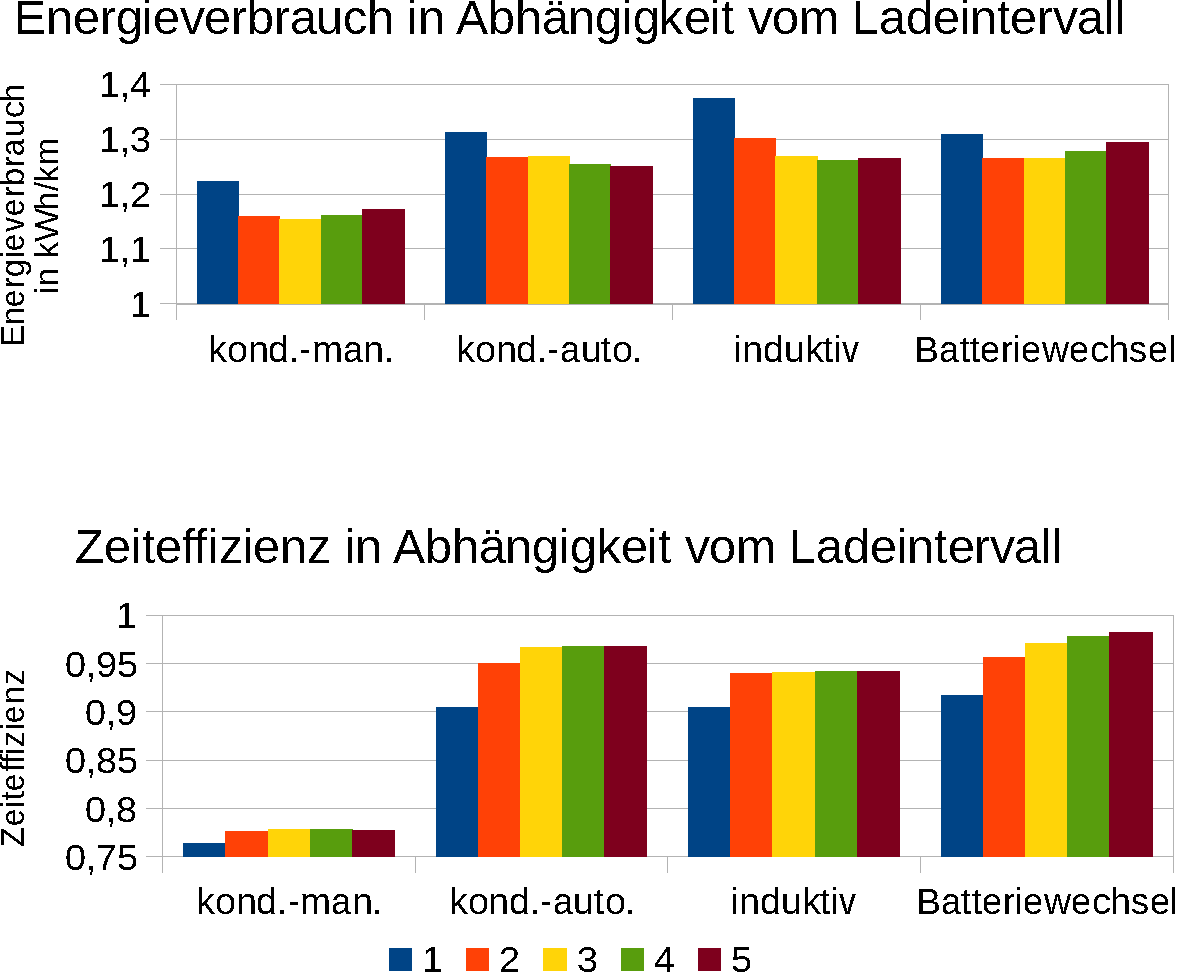
\includegraphics[width=\myFigureStandardWidth]{DiagrammeLadeintervall}
	\caption[Zeiteffizienz und Energieverbrauch für verschiedene Ladeintervalle]{Zeiteffizienz und Energieverbrauch für verschiedene Ladeintervalle. Die unterschiedlichen Farben zeigen die Werte, wenn der Bus nach jedem n-ten Umlauf aufgeladen wird. Es wurde ein Lithium-Titanat-Akku auf der Linie 204 verwendet.}
	\label{abb_DiagrammLadeintervalle}
\end{figure}

In einer wirtschaftlichen Analyse sollte untersucht werden, bei welchem Ladeintervall die Kombination von Investitionskosten für die Batterie und laufenden Kosten für den Bus minimiert wird. 

\subsection{Simulation der Batterielebensdauer}
Im Rahmen der Simulation wurde in dieser Arbeit die Anzahl der Ladezyklen pro Kilometer für die verschiedenen Kombinationen von Batterie und Ladesystem berechnet. Daneben habe aber auch Temperatur, durschschnittliche Entladetiefe sowie Lade- und Entladestrom einen Einfluss auf die Lebensdauer. Es bietet sich an, mithilfe von aufgezeichneten Fahrstrecken an verschiedenen Tageszeiten sowie einem Klimatisierungsmodell für das ganze Jahr die Lebensdauer der verschiedenen Kombinationen genauer zu berechnen. Für Lithium-Eisenphosphatbatterien haben Lam und Bauern~\cite{lam2013practical} bereits ein empirisches Modell zur Berechnung der Lebensdauer geschaffen, das in das existierende Simulationsmodell eingebunden werden kann.

\subsection{Wiederverwendung alter Batterien auf kürzeren Linien}
Batterien für Elektrofahrzeuge gelten als aufgebraucht, wenn sie nur noch 80\% ihrer ursprünglichen Ladung speichern können. Da sich der Energieverbrauch je nach Buslinie unterscheidet können jedoch Batterien, die für lange Buslinien nicht mehr geeignet sind, auf kürzeren Buslinien noch erfolgreich eingesetzt werden. Das Einsparpotenzial einer solchen Wiederverwendung von Batterien aus technischer und wirtschaftlicher Sicht sollte weiter analysiert werden.

\subsection{Zusammengefasstes Temperaturmanagement}
In aktuellen Bussen werden separate Kühl- und Heizkreisläufe für Batterie und Innenraum verwendet. Damit werden einerseits Komponenten doppelt verbaut, andererseits kann es vorkommen das die Batterie gekühlt wird während der Fahrgastraum geheizt wird, so dass Energie verschwendet wird. Ein gemeinsames Temperierungssystem für Innenraum und Batterie würde die Fahrzeugmasse reduzieren und die Energieeffizienz ggf. stark erhöhen.

\subsection{Verbesserung der Ladeleistung}
Ergebnis der hier durchgeführten technischen Analyse ist, das die \emph{Entladeleistung} der aktuellen Batterien in allen betrachteten Fällen ausreicht. Durch die begrenzte \emph{Ladeleistung} geht jedoch einerseits Rekuperationsleistung verloren, andererseits steigt die Ladedauer. Eine Erhöhung der spezifischen Ladeleistung verbessert die Attraktivität von Elektrobussen weit mehr als eine vergleichbare Verbesserung der spezifischen Energie oder Entladeleistung. Zur Verbesserung der Rekuperationsleistung bietet sich der Einsatz eines hybriden Speichersystems mit leistungsstarken Superkondensatoren und energiereichen Batterien an. Wie groß der Vorteil eines solchen Systems wäre, kann durch eine Erweiterung des bestehenden Simulationsmodells berechnet werden.